% !TEX root SCHISADCJPOA JPFDÈOC KJ+ÒLDkc= ../Thesis.tex

\chapter{ORGANIZZAZIONE DATASET DELLA RETE NEURALE PER LA MAPPA DI QUALITÀ}

\begin{figure}[h] % [h] = here, posiziona dove possibile
    \centering
    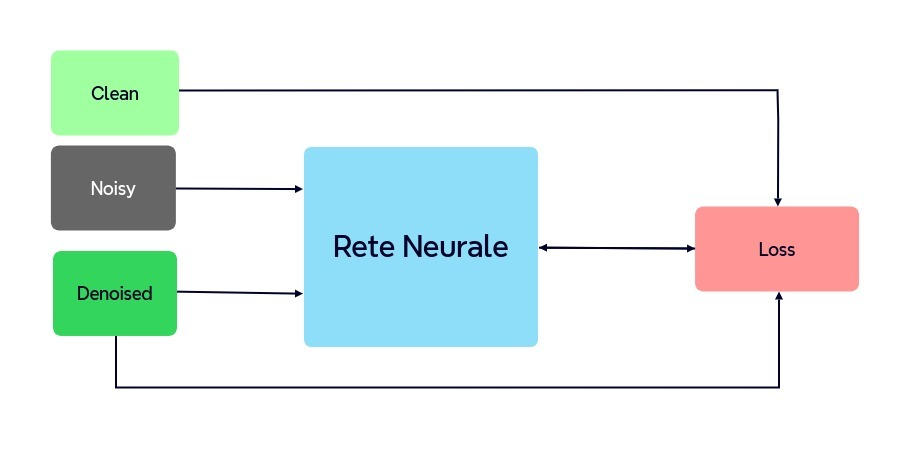
\includegraphics[width=0.8\textwidth]{utils/Architettura_rete_neurale.jpg}
    \caption{Mock della struttura della rete neurale per la previsione della qualità}
    \label{fig:MockReteNeurale}
\end{figure}

Come illustrato in Figura \ref{fig:MockReteNeurale}, il dataset impiegato è costituito da tre tipologie di 
immagini: clean, noisy e denoised. Queste immagini sono state realizzate tramite uno strumento ottico di un
satellite per poi essere sporcate con speckle artificiale e su cui infine è stato fatto denoising. Questa scelte è stata fatta
in quanto risulta difficile reperire un dataset contenente immagini SAR abbastanza grande per poter 
addestrare una rete neurale. Le immagini su cui viene fatto l'addestramento sono relative ad un singolo modello di despeckling ed ad 
un determinato look. Quest'ultimo è una metrica che indica l'intensità dello speckle artificiale, in quanto a più look 
corrispondono più catture di quella che è la realtà di interessa e quindi si ha una maggior precisione e uno speckle ridotto.
In fase di addestramento, le immagini noisy e denoised vengono concatenate in un unico tensore a due canali e utilizzate come 
input per la rete neurale. Le immagini clean, invece, assieme a quelle denoised, vengono impiegate per la 
generazione della mappa di qualità, che costituisce il riferimento necessario per 
il calcolo della funzione di perdita. Questo permette al modello di imparare a 
prevedere la qualità del denoising relative ad un dato modello di despeckling e ad determinato   